\documentclass[11pt,class=article,float=false,crop=false]{standalone}
\usepackage{Part1_packages}

\begin{document}

\section{Simulation numérique avec OptiDis}

La Dynamique des Dislocations est utilisée pour effectuer des simulations afin de modéliser le comportement mécanique des matériaux. Le livre de \textsc{V. Bulatov}\citebiblio{bulatov2006computer} offre une vue d'ensemble des simulations autour de la Dynamique des dislocations. Nous nous intéresserons particulièrement à la Dynamique des Dislocations Discrète utilisée dans le simulateur OptiDis.

%Computer simulations of dislocations - Bulatov

\subsection{Dynamique des Dislocations Discrète}

Dans Dynamique des Dislocations Discrète (DDD), les lignes de dislocation sont discréditées afin de résoudre numériquement par un formalisme éléments finis leur déplacement. Nous expliquerons les principes de la discrétisation des dislocation en prenant l'exemple du code OptiDis. Nous nous intéresserons ensuite aux codes qui forment l'écosystème de la simulation de Dynamique des Dislocations.

\subsubsection{Modèle de discrétisation des dislocations}

Dans OptiDis, nous utilisons une représentation nodale des dislocations. Le réseau de dislocations est représenté par un ensemble de nœuds connectés par des segments qui portent des propriétés telles que le système de glissement auxquels ils appartiennent. Les segments peuvent être orientés dans toutes les directions, permettant de modéliser des dislocations mixtes. La figure \ref{fig:representation_nodale} représente un réseau de dislocation discrétisé avec une représentation nodale.

\begin{figure}[H]
	\centering
	\includetikz[0.5]{img/dislocation-discrete}
	\caption{Représentation nodale d'un réseau de dislocations.}
	\label{fig:representation_nodale}
\end{figure}

Dans cette représentation, la notion de nœud topologique apparaît. Il s'agit des nœuds blancs qui, contrairement aux nœuds physiques en noir, n'ont pas de signification physique. Ce sont des nœuds de discrétisation qui forment les segments. Nous verrons par la suite que des interactions entre les segments sont calculées pour déterminer le déplacement de ces nœuds.


\subsubsection{Ecosystème}

Les premières simulations de Dynamiques des Dislocations, telles que Tridis (CEA) et Micromegas (CNRS-ONERA) utilisaient une approche par segments. Le réseau était représenté par une ligne brisée contenant des dislocations vis/coins. L'approche nodale utilisant des dislocations mixtes \citebiblio{kuktat1998three} est utilisée dans les codes plus récents tels que Model (UCLA), Paradis (Stanford), Numodis/OptiDis (CEA). La différence entre l'approche nodale et l'approche vis/coin est illustrée dans le figure \ref{fig:modelisation_vis_coin}. Le modèle vis/coin est plus rapide, mais ne permet pas de simuler de manière précise certains phénomènes comme la formation de jonctions.

\begin{figure}[H]
	\centering
	\begin{subfigure}[b]{0.49\textwidth}
		\centering
		\includetikz[0.65]{img/discretisation-vis-coin}
		\caption{Modèle Vis/Coin}
	\end{subfigure}
	\begin{subfigure}[b]{0.49\textwidth}
		\centering
		\includetikz[0.70]{img/discretisation-mixte}
		\caption{Dislocations mixtes}
	\end{subfigure}
	\caption{Différentes modélisations des dislocations.}
	\label{fig:modelisation_vis_coin}
\end{figure}

Des approches nodales ont été mises en places pour observer les phénomènes d'écrouissage avec le code ParaDis \citebiblio{bulatov2006nature} et le durcissement lié à l'irradiation avec NumoDis \todo[inline]{source : durcissement irradiation Numodis?}. Ces codes nécessitent une puissance de calcul importante et évoluent donc vers des codes de simulation massive sur des supercalculateurs. NumoDis devient alors OptiDis en évoluant vers les architectures parallèles \citebiblio{etcheverry2015simulation}.

\subsection{Déroulement de la simulation}
\label{sec:etapes_simulation}

Lors d'une simulation de Dynamique des Dislocations, plusieurs itérations sont effectuées pour déplacer les segments de dislocation. Au cours de chaque itération, le calcul se divise en plusieurs étapes. Dans cette section, nous verrons quelle sont les étapes d'une itération. Nous verrons en particulier comment se déroulent les étapes du calcul des forces, et du déplacement des dislocations.

\subsubsection{Vue d'ensemble}

La figure \ref{fig:deroulement_simulation} illustre les différentes étapes de la simulation et leurs dépendances en données.

\begin{figure}[H]
	\centering
	\includetikz{img/etapes-simulation}
	\caption{Les étapes de la simulations dans OptiDis.}
	\label{fig:deroulement_simulation}
\end{figure}

Les itérations déplacent les dislocations en effectuant les actions suivantes :

\paragraph{Calcul des forces : }
La première étape consiste à calculer les forces $F_t$ appliquées sur les nœuds. Les forces nodales dépendent principalement des positions des noeuds au temps courant $P_t$ et des propriétés des segments de dislocation telles que le vecteur de Burgers. Les formules analytiques d'Arsenlis sont utilisées pour le calcul des forces. Cette étape est très gourmande en calcul, et la Méthode des Multipoles Rapide (FMM) est utilisée pour l'accélérer. 

\paragraph{Mobilité : }

Les vitesse nodales $V_t$ sont calculées en fonction des forces appliquées sur les nœuds mais aussi de leur système de glissement. 

\paragraph{Déplacement : }

Les nœuds sont déplacés à une position prédictive $P^\prime$ qui ne prend pas en compte les opérations locales comme les collisions. Cette étape consiste à intégrer la vitesse au cours du temps pour obtenir une nouvelle position.

\paragraph{Opérations locales : }
Les opérations locales modifient le réseau de dislocation pour prendre en compte certains phénomènes comme la formation de jonctions. Lors de cette étape, le réseau de dislocations est raffiné pour que les différents segments qui le compose possèdent une longueur homogène.

\paragraph{}
Entre les différentes étapes peuvent être intercalées des étapes d'affichage ou d'enregistrement de certains résultats de simulation.


\subsubsection{Calcul des forces nodales.}
\label{sec:forces_nodales}

Le calcul des forces nodales se base sur la force de Peach-Koheler \citebiblio{peachkoehler1950forces} (équation \ref{eq:Peach-Koheler}). En plus des forces exercées par les contraintes externes, les dislocations subissent des forces internes induites par les autres dislocations. 

La formulation de Mura \citebiblio{mura2013micromechanics} pose la base du calcul du champs de contraintes généré par une ligne de dislocation $L$:

\begin{equation}
\sigma^L_{ij} (x) = C_{ijkl} \int_L \epsilon _{lnh} C_{pqmn} G_{kp,q} (x-x')b_m dx'_h
\end{equation}

\begin{itemize}
	\item $\sigma$ le tenseur des contraintes élastiques;
	\item $C_{ijkl}$ le tenseur des constantes élastiques qui intervient dans l'expression de la loi de Hooke généralisée aux matériaux anisotropes;
	\item $\epsilon _{lnh}$ le symbole de Levi-Civita;
	\item $G_{kp,q} (x-x')$ est la fonction de green définie par Mura \citebiblio{mura2013micromechanics}. Elle représente le déplacement dans la direction $x_k$ au point $x$ en réponse à la force dans la direction $x_p$ appliquée au point $x'$ de la dislocation. 
	\item b le vecteur de burgers.
\end{itemize}

Pour obtenir la force appliquée par le segment $S_j$ sur $S_i$ ($f_{ij}$), il faut intégrer $\sigma$ sur $S_j$ puis la force de Peach-Koheler sur $S_i$:

\begin{equation}
\vect{f}_{ij} = \int_{S_i} (\tensor{\sigma}^{S_j} \cdot \vect{b}) \times \vect{\xi}
\end{equation}

Des formules analytiques existent pour le calcul de $\vect{f}_{ij}$ \citebiblio{arsenlis2007enabling}. L'intégration analytique permet de calculer la force plus rapidement qu'avec une intégration numérique. Cependant, les formules analytiques nécessitent d'utiliser la théorie non-singulière, qui nécessite d'ajouter une force de cœur pour les interactions à faible distance (tension de ligne, ...).

Enfin, pour calculer la force appliquée sur chaque segment $\vect{F}_i$ , il faut sommer les contributions de chaque autre segment:

\begin{equation}
\vect{F}_i = \sum_{j} \vect{f}_{ij}
\label{eq:force_nodale}
\end{equation}

La force nodale est calculée en prenant en compte les forces appliquées sur les segments connectés au nœud considéré.

La complexité quadratique de cette étape en fait l'étape la plus coûteuse de la simulation. Nous verrons dans la partie \ref{sec:FMM} quelles solutions ont été mises en place pour accélérer le calcul.

%Thèse de Pierre?

\subsubsection{Déplacement des dislocations}

Une fois le calcul des forces terminé, les nœuds doivent être déplacés. La vitesse de chaque nœud doit être déterminée, puis intégrée pour obtenir la nouvelle position

\paragraph{Calcul des vitesses nodales.}

La vitesse en tout point $\vect{v}(\vect{x})$ du réseau de dislocation est interpolée linéairement en fonction des vitesses $\vect{v}_i$ des noeuds:
\begin{equation}
\vect{v}(\vect{x})  = \sum_{i=1}^N N_i(\vect{x}) \vect{v}_i(\vect{x})
\label{eq:mobility_interp}
\end{equation}

Avec $N_i$ une fonction qui décroît linéairement de 1 à 0 le long des segments connectés au nœud $i$ à la position $x_i$:
\begin{equation}
N_i(\vect{x}) = \left\{
\begin{array}{ll}
\frac{||\vect{x} - \vect{x}_j||}{||\vect{x}_i-\vect{x}_j||} & \text{si } x \in [x_i,x_j] \\
0 															& \text{sinon}\\
\end{array}
\right. 
\end{equation}

Les lois de mobilité définissent la vitesse d'un élément infinitésimal de dislocation en fonction des forces qui lui sont appliquées:
\begin{equation}
\vect{v}(\vect{x}) = M(\vect{f}(\vect{x}))	
\end{equation}


Le modèle choisi est le glissement visqueux linéaire quasi-statique où $\tensor{\mathcal{B}}$ est un tenseur qui pourra dépendre de la nature des dislocations considérées \footnote{Dépend en fait de $\vect{x}$ mais est constant le long d'un segment de dislocation. Pour éviter la notation trompeuse $\tensor{\mathcal{B}(\vect{x})}$, on omet la dépendance en $\vect{x}$.}
\begin{equation}
	\tensor{\mathcal{B}} \cdot \vect{v}(\vect{x}) = \vect{f}(\vect{x})	
\end{equation}

Les vitesses nodales sont résolues par la méthode des éléments finis. La formulation variationnelle sur le réseau de dislocation $\mathcal{D}$  s'écrit:
\begin{equation}
\int_\mathcal{D} \tensor{\mathcal{B}}  \vect{v}(\vect{x}) N_i(\vect{x})  d\vect{x} = \int_\mathcal{D} \vect{f}(\vect{x}) N_i(\vect{x}) d\vect{x}
\label{eq:formulation_variationnelle}
\end{equation}

Les fonctions les fonctions test $N_i$ sont décrites dans l'équation \ref{eq:mobility_interp}.

La formulation variationnelle se simplifie en le système linéaire suivant:
\begin{equation}
\vect{B}\vect{v} = \vect{f}
\label{eq:mobilite_systeme}
\end{equation}

\begin{itemize}
	\item Les coordonnées $v_i$ de $v$ sont les vitesses nodales de l'équation \ref{eq:mobility_interp}.
	\item Les coordonnées $f_i$ de $f$ sont les forces nodales calculées en section \ref{sec:forces_nodales} dont l'expression est la partie gauche de l'équation (\ref{eq:formulation_variationnelle}).
	\item $\vect{B}$ une matrice $N\times N$ dont les coefficients à valeurs tensorielles s'expriment:
\end{itemize}

\begin{equation}
	\tensor{B_{ij}} = \int_\mathcal{D} N_i(\vect{x}) N_j(\vect{x}) \tensor{\mathcal{B}} d\vect{x}
\end{equation}

Il est intéressant de noter que $\tensor{B_{ij}}$ est nul lorsque les noeuds $i$ et $j$ ne sont pas connectés. La matrice $\vect{B}$ est donc une matrice creuse. Il est possible de résoudre le système explicitement, mais cela est très couteux. Une simplification \citebiblio{bulatov2006computer} permet d'obtenir une vitesse nodale de manière locale:

\begin{equation}
\vect{v}_i \approx \frac{\vect{f}_i}{B\sum_{j\text{ connecté à } i } L_{ij}}
\end{equation}





\paragraph{Calcul de la nouvelle position.}
Une fois la vitesse trouvée, il faut intégrer la vitesse pour déterminer le déplacement:

\begin{equation}
p(t+\Delta t) = p(t) + \int_{\tau=t}^{d+\Delta t} v(\tau) d\tau
\end{equation}

La solution la plus simple est de considérer la vitesse constante au cours du pas de temps:

\begin{equation}
p(t+\Delta t) = p(t) + v(t)\Delta t
\end{equation}

Cependant cette méthode d'ordre 1 nécessite un pas de temps très court pour être stable. Des intégrateurs prédicteur-correcteur peuvent aussi être utilisés \citebiblio{sills2016advanced}. L'ordre d'un tel intégrateur est plus élevé, et reste stable pour des pas de temps plus grands. Le nombre de pas de temps à effectuer pour la même simulation serait moindre, mais chacun serait plus coûteux. Il y a ici un compromis à trouver entre précision et rapidité pour l'intégrateur.

%Advanced time integration algorithms -- RB Sillis

\subsubsection{Opérations locales}

Lorsque deux lignes de dislocations en mouvement entrent en contact, il peut y avoir ou non formation d'une jonction. Les jonctions jouent un rôle important dans de nombreux phénomènes, comme par exemple le durcissement par irradiation. Cependant, les opérations basées sur les interactions entre dislocations vues précédemment ne peuvent pas gérer la formation de ces jonctions. Des opérations locales se chargent d'effectuer les changements topologiques nécessaires à la formation de jonctions. 

Les opérations locales se déroulent en deux phases principales. Premièrement, une gestion des collisions doit être effectuée pour fusionner les dislocations qui entrent en contact. Ensuite une opération nommée \textit{splitnode} permet de choisir parmi plusieurs configurations possibles lors d'un contact.

\paragraph{Gestion des collisions}

La première étape consiste à détecter si des segments de dislocation entrent en contact avec d'autres dislocations, ou avec d'autres objets comme des pécipités ou des joints de grain. Ensuite, il faut appliquer des transformations topologiques pour fusionner les dislocations qui entrent en contact. Le but est d’effectuer le déplacement des segments sans qu'ils ne se traversent mutuellement.

Les mécanismes de gestion des collisions font l'objet des travaux présentés dans la partie \ref{part:collision}.

\paragraph{SplitNode}

La formation de jonctions est un phénomène complexe, et la topologie qui résulte du contact entre deux dislocations dépend beaucoup de la nature de celles-ci \citebiblio{bulatov2006nature,terentyev2008simulation,shi2014these}. Parmi les configurations possibles, la configuration qui apparaît en réalité est celle qui nécessite le moins d'énergie pour sa formation. Le principe de cette opération est de calculer l'énergie nécessaire à la formation de plusieurs types de jonctions, et de choisir la configuration la plus favorable.

Lorsqu'un nœud physique est connecté à plus de 2 segments, il peut être plus favorable énergétiquement que ce nœud soit scindé en deux pour former une jonction. La figure \ref{fig:configurations_jonctions} énumère quelques configurations possibles pour la formation d'une jonction au niveau d'un nœud physique de degré 4.

\begin{figure}[H]
	\centering
	\includetikz[1.2]{img/possibilites-splitnode}	
	\caption{Configurations possibles lors de la formation de jonctions.}
	\label{fig:configurations_jonctions}
\end{figure}


\subsection{Considérations informatiques}

OptiDis s'inscrit dans un projet de simulation massivement parallèle de Dynamique des Dislocations. Il est donc incontournable de s'intéresser aux aspects liés à la complexité algorithmique des opérations effectuées, ainsi qu'a la manière d'exploiter des ordinateurs massivement parallèles. 

\subsubsection{Complexité}

Les opérations les plus coûteuses au cours de la simulation sont celles qui font intervenir des interaction entre les segments et entre les noeuds, comme le calcul des forces et la détection des collisions. Estimons par exemple la complexité du calcul des forces élastiques : 


On souhaite calculer la force $F_i$ pour chacun des $N$ segments du réseau de dislocations:

\begin{equation}
	C_{force} = N*C_{F_i}
\end{equation}

Pour chaque $F_i$, il faut calculer et sommer la contribution de chaque autre segment $f_{ij}$ selon la formule (\ref{eq:force_nodale}) :

\begin{equation}
   C_{F_i} = (N-1)*C_{f_{ij}}
\end{equation}

Les contributions $f_{ij}$ sont calculées à partir des formules analytiques qui, bien que longues à calculer, se calculent en temps constant:

 \begin{equation}
 C_{f_{ij}} = O(1)
 \end{equation}
 
En combinant ces résultats, on obtient que le calcul des forces possède une complexité quadratique en fonction du nombre de segments:

\begin{equation}
C_{force} = N(N-1)C_{f_{ij}} = O(N^2)
\end{equation}

Une telle complexité est problématique car le temps de calcul explose lorsque l'on souhaite augmenter le nombre segments de dislocations.

\subsubsection{Fast Multipole Method}
\label{sec:FMM}

Le calcul des forces élastiques s'apparente au problème à N corps, pour lequel des solutions algorithmiques ont été développées afin de réduire sa complexité. Parmi ces solutions, la méthode des multipôles rapides découpe l'espace de manière hiérarchique pour effectuer des approximations de champs lointains.

\paragraph{Partitionnement de l'espace}

La FMM se base sur un découpage hiérarchique de l'espace selon un octree. Chaque boite est successivement découpée en 8 dans le cas de la dimension 3. La figure \ref{fig:FMM:octree} illustre le découpage du plan selon un quadtree.

\begin{figure}[H]
	\centering
	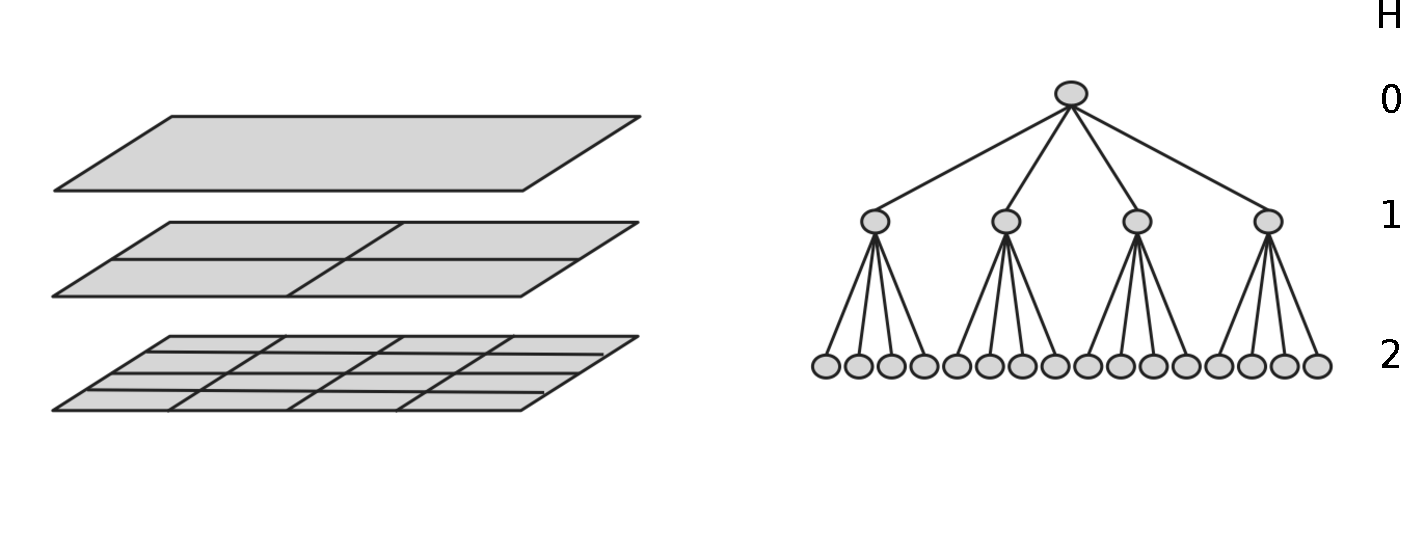
\includegraphics[width=\textwidth]{img/fmm-octree}
	\caption{Découpage du plan en boites FMM.}
	\label{fig:FMM:octree}
\end{figure}

Les boites du niveau le plus bas appelées feuilles contiennent les particules, et les nœuds des autre niveaux appelés cellules contiennent des développement multipolaires.

\paragraph{Développements multipolaires.}

Les développement multipolaires représentent la contributions des particules contenues dans une cellule au champ lointain. Il s'agit en quelques sorte d'une particule équivalente à l'ensemble des particules contenues dans la cellule. Lorsque deux cellules sont suffisamment éloignées, on pourra remplacer les calcul des interactions entre toutes les particules des deux boites par l'application d'un multipôle, comme l'illustre la figure \ref{fig:fmm:multipole}.

\begin{figure}[H]
	\centering
	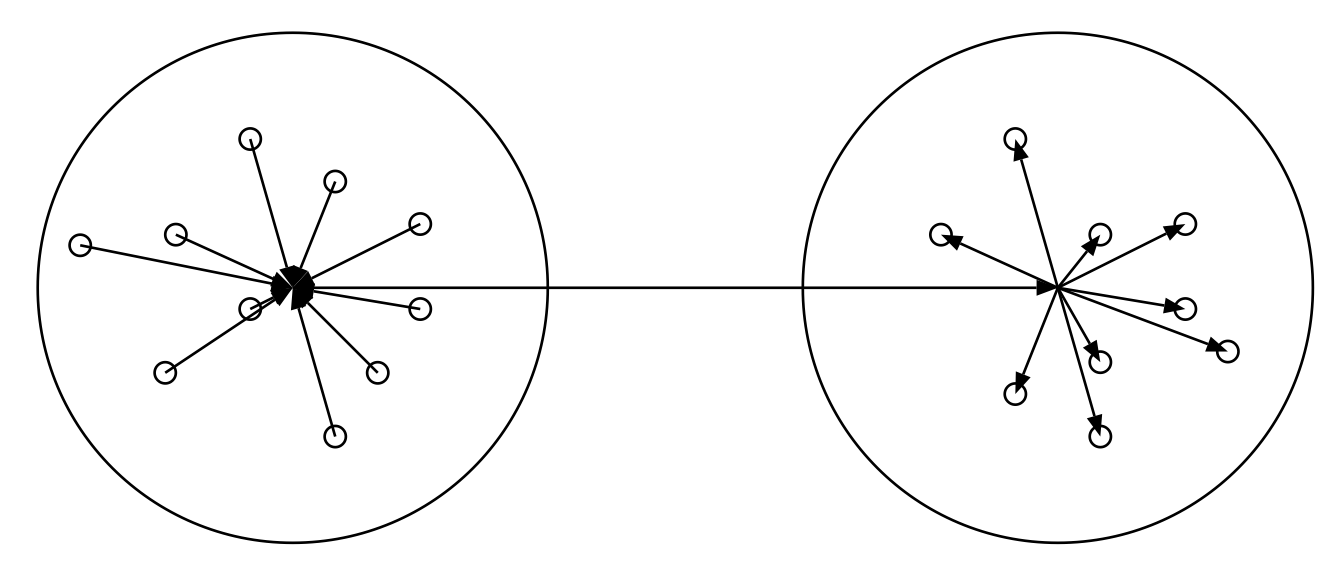
\includegraphics[width=0.8\textwidth]{img/fmm-multipole}
	\caption{L'application d'un multipôle pour calculer le champ lointain.}
	\label{fig:fmm:multipole}
\end{figure}

Des développements multipolaires sont portés par toutes les cellules, à toutes les échelles de raffinement. La méthode des multipôles rapides est donc une méthode hiérarchique. Pour chaque feuille et cellule, on distingue deux calculs : le champs proche et le champs lointain. 

Le champ proche est l'interaction entre les particules proches. à un niveau de raffinement donné, le voisinage direct d'une boite est constitué des boites au même niveau de raffinement qui sont en contact direct, comme l'illustre la figure \ref{fig:fmm:voisin}. Les interactions entre les particules de boites voisines sont calculées de manières exactes (P2P).

\begin{figure}[H]
	\centering
	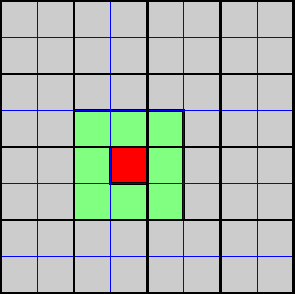
\includegraphics[height=0.2\textheight]{img/fmm-voisins}	
	\caption{Voisins directs d'une boite.}
	\label{fig:fmm:voisin}
\end{figure}

Les autres feuilles et boites constituent le champ lointain dont le calcul est approximé par le développement multipolaire.


\subsubsection{Structures de données}

La différence majeure entre la Dynamique des Dislocations et le problème à N corps est le caractère dynamique du nombre de particules considéré. A l'inverse du problème à N corps où un nombre fixé de particules entrent en interaction, le nombre d'objets dans la Dynamique des Dislocations évolue au cours du temps. Les opérations topologiques telles que les collisions ou le raffinement du maillage peuvent ajouter ou retirer des nœuds et des segments du réseau de dislocations. Le caractère dynamique des données pose un défi majeur pour la performance des simulations massives.

\paragraph{}
La cohérence spatiale et temporelle est une base des principes d'accès aux données. Les architectures matérielles des ordinateurs sont optimisées pour accéder à des données stockées proche les unes des autres, et permettent un accès plus rapide aux données contiguës et récemment utilisées. La cohérence spatiale et temporelle apparaît naturellement dans de nombreux algorithmes, mais nécessite parfois d'adapter l'ordre d'accès aux données pour l'obtenir. Il s'agit la plus part du temps de trier la mémoire pour accéder dans l'ordre aux éléments souhaités.

Par exemple, dans la FMM, les particules sont triées afin que celles qui sont proches dans l'espace le soient aussi en mémoire. On utilise une \textit{space-filling curve} comme la Z-curve illustrée figure \ref{fig:z-curve} qui permet de linéariser l'espace pour obtenir une relation d'ordre totale qui garantit une meilleure cohérence spatiale des données. L'espace est découpé en boites numérotées selon leur ordre sur la Z-curve, appelé indice de Morton. Les particules sont rangées par boites et rangées selon leur indice de Morton. 

\begin{figure}[H]
	\includetikz{img/z-curve}	
	\caption{Z-curve}
	\label{fig:z-curve}
\end{figure}

\paragraph{}
Lorsque les données sont dynamiques, c'est à dire que le nombre d'objets n'est pas constant, la cohérence spatiale des données est difficile à maintenir. Les structures de données utilisées doivent alors être optimisées pour un certain cas d'usage. Faut-il que les données insérées respectent la cohérence spatiale au prix d'une insertion plus coûteuse, ou au contraire faut-il pouvoir insérer rapidement un élément en sacrifiant la cohérence spatiale.

Par exemple pour la FMM, il existe plusieurs manières de stocker les particules de manière à ce qu'elles soient triées par boites : 
\begin{itemize}
	\item Chaque boite est représentée par un tableau de particules indépendant : Insérer une particule dans sa boite est simple, mais la cohérence spatiale est faible car il faut faire un saut en mémoire entre les boites pour parcourir toutes les particules.
	\item Toutes les particules sont stockées dans un unique tableau trié en fonction de l'indice de Morton de chaque particule : La localité spatiale est très bonne, mais l'insertion est très coûteuse. Pour insérer une particule, il faut décaler toutes celles à sa droite.
\end{itemize}

Le nombre de segments dans la Dynamique des Dislocations varie beaucoup au cours du temps. Les opérations topologiques de formation de jonctions et de remaillage créent et suppriment des nœuds et des segments. Afin d'obtenir un bon compromis entre localité et vitesse d'insertion, des structures de données dynamiques ont été mises en œuvre dans OptiDis au cours de la thèse de A. Etcheverry \citebiblio{etcheverry2015simulation}.

\end{document}	